\documentclass[a4paper,11pt]{article}
\input{/home/tof/Documents/Cozy/latex-include/preambule_doc.tex}
\input{/home/tof/Documents/Cozy/latex-include/preambule_commun.tex}
\newcommand{\showprof}{show them}  % comment this line if you don't want to see todo environment
\setlength{\fboxrule}{0.8pt}
\fancyhead[L]{\fbox{\Large{\textbf{Routage 07}}}}
\fancyhead[C]{\textbf{Exercices - plus court chemin}}
\newdate{madate}{10}{09}{2020}
%\fancyhead[R]{\displaydate{madate}} %\today
%\fancyhead[R]{Seconde - SNT}
%\fancyhead[R]{Première - NSI}
\fancyhead[R]{Terminale - NSI}
\fancyfoot[L]{\vspace{1mm}Christophe Viroulaud}
\AtEndDocument{\label{lastpage}}
\fancyfoot[C]{\textbf{Page \thepage/\pageref{lastpage}}}
\fancyfoot[R]{\includegraphics[width=2cm,align=t]{/home/tof/Documents/Cozy/latex-include/cc.png}}
\usepackage{tikz}

\begin{document}
\begin{center}
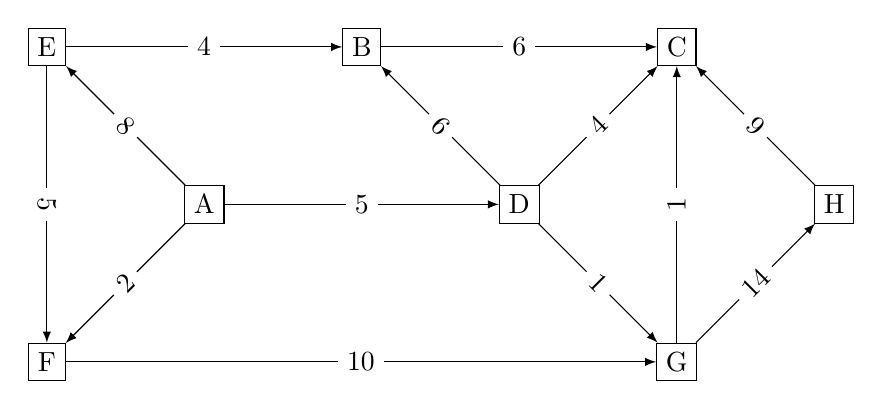
\begin{tikzpicture}[scale=2]
    \node[draw] (A) at (1,1) {A};
    \node[draw] (B) at (2,2) {B};
    \node[draw] (C) at (4,2) {C};
    \node[draw] (D) at (3,1) {D};
    \node[draw] (E) at (0,2) {E};
    \node[draw] (F) at (0,0) {F};
    \node[draw] (G) at (4,0) {G};
    \node[draw] (H) at (5,1) {H};

    \draw[->,>=latex] (A)--(F) node[sloped, midway, fill=white]{2};
    \draw[->,>=latex] (A)--(E) node[sloped, midway, fill=white]{8};
    \draw[->,>=latex] (E)--(F) node[sloped, midway, fill=white]{5};
    \draw[->,>=latex] (A)--(D) node[sloped, midway, fill=white]{5};
    \draw[->,>=latex] (E)--(B) node[sloped, midway, fill=white]{4};
    \draw[->,>=latex] (F)--(G) node[sloped, midway, fill=white]{10};
    \draw[->,>=latex] (D)--(B) node[sloped, midway, fill=white]{6};
    \draw[->,>=latex] (B)--(C) node[sloped, midway, fill=white]{6};
    \draw[->,>=latex] (D)--(C) node[sloped, midway, fill=white]{4};
    \draw[->,>=latex] (D)--(G) node[sloped, midway, fill=white]{1};
    \draw[->,>=latex] (G)--(C) node[sloped, midway, fill=white]{1};
    \draw[->,>=latex] (G)--(H) node[sloped, midway, fill=white]{14};
    \draw[->,>=latex] (H)--(C) node[sloped, midway, fill=white]{9};
\end{tikzpicture}
\end{center}
En partant de A:
\begin{enumerate}
    \item Appliquer l'algorithme de Bellman-Ford sur le graphe.
    \item Appliquer l'algorithme de Dijkstra sur le graphe.
\end{enumerate}
\end{document}